% Kompiuterijos katedros šablonas
% Template of Department of Computer Science II
% Versija 1.0 2015 m. kovas [ March, 2015]

\documentclass[a4paper,12pt,fleqn]{article}
\usepackage[unicode,colorlinks=false]{hyperref}


\usepackage[utf8x]{inputenc}
%

\usepackage[L7x]{fontenc}
\usepackage{times}
\usepackage{ucs}

 %package to switch the language
\usepackage{etoolbox}

  %set up of the page margins
\usepackage[top=2cm, bottom=2cm, left=3cm, right=1.5cm]{geometry}

 %1.1 line spacing
\linespread{1.1}


  %page numbering at the right side
\usepackage{fancyhdr}
\pagestyle{fancyplain}
\fancyhf{}
\renewcommand{\headrulewidth}{0pt} 
\fancyhfoffset[RO]{0cm}

  %to number at the bottom (exchange lines to number at the top)
\rfoot{\thepage}
  %\rhead{\thepage} %

% \usepackage[usenames,dvipsnames]{pstricks}
\urlstyle{same}
\hypersetup{
%  citecolor=Blue,
%  linkcolor=Blue,
%  urlcolor=Blue
pdfborder={0 0 0 }
}

 %for includegraphics
\usepackage{graphicx}



\usepackage[toc,page]{appendix}


\usepackage{caption}

 %for source codes
\usepackage{listings}
\lstset{commentstyle=\color{red},xleftmargin=10pt, framexleftmargin=6pt, numbersep=1mm, frame=single, numbers=left,numberstyle=\footnotesize,extendedchars=\true, inputencoding=utf8x,basicstyle=\footnotesize,extendedchars=true,
 keywordstyle=\color{black}\bfseries, breaklines=true, breakautoindent=true,framesep=8pt,linewidth=0.95\textwidth
}

 %for algorithms
\usepackage{algorithm}
\usepackage{algorithmic}
 %instead of the above two packages we can use algorithms2e
 %\usepackage[boxed,linesnumbered,vlined,slide]{algorithm2e}

 %special symbols
\usepackage{amsfonts}
\usepackage{amssymb}
\usepackage{amsmath}

 %for theorem like environments
\usepackage{amsthm}

 \usepackage{datetime}
 \renewcommand{\dateseparator}{--}


% SI system units
\usepackage{siunitx}
\sisetup{detect-all}
% Problem with fonts \SI{x.xx}{\micro\metre}, solved with updmap-sys --enable Map=utm.map
\renewcommand{\sfdefault}{uhv}
\renewcommand{\rmdefault}{utm}
\renewcommand{\ttdefault}{ucr}

% List management (itemize, etc.)
\usepackage{enumitem}

\newcommand*{\urlw}[1]{\href{#1}%
            {\nolinkurl{#1}}}

\numberwithin{equation}{section}

\graphicspath{ {Pav/} }
\usepackage{graphicx}
\usepackage{subcaption}
\usepackage{listings}
\captionsetup{font=small,labelfont=it,textfont=it}
\lstset{numbers=left, numberstyle=\tiny, stepnumber=1, language=Java, captionpos=b, frame=single, aboveskip=20pt,belowskip=20pt }

\newtoggle{inLithuanian}
 %If the report is in Lithuanian, it is set to true; otherwise, change to false
\settoggle{inLithuanian}{true}

%create file preface.tex for the preface text
%if preface is needed set to true
\newtoggle{needPreface}
\settoggle{needPreface}{false}

\newtoggle{signaturesOnTitlePage}
\settoggle{signaturesOnTitlePage}{true}


\theoremstyle{definition}
\newtheorem{definition}{\keyWordDefinition}
\newtheorem{example}{\keyWordExample}
\def\QED{\unskip\nobreak\hfill\kern5pt$\Box$}

\iftoggle{inLithuanian}{
%\usepackage[L7x]{fontenc}
\usepackage[english,lithuanian]{babel}

\newcommand{\todayiso}{\the\year \dateseparator \twodigit\month \dateseparator \twodigit\day}


\renewcommand{\today}{\number\year\space m. \space \ifcase\month\or
  sausio\or vasario\or kovo\or balandžio\or gegužės\or birželio\or
  liepos\or rugpjūčio\or rugsėjo\or spalio\or lapkričio\or
  gruodžio\fi
  \space\number\day\space d.}


 \usepackage{tocloft}
 \renewcommand\cftsecaftersnum{.} 
 \renewcommand\cftsubsecaftersnum{.} 
 \renewcommand\cftsubsubsecaftersnum{.}

 \usepackage{VUMIFKK}

 \DeclareCaptionLabelFormat{captionlt}{#2 #1}
   %smth is not fine with algorithms 
 \DeclareCaptionLabelFormat{captionltalg}{#2 #1 algoritmas}

 \usepackage{indentfirst}
 \renewcommand{\appendixtocname}{Priedai}
 \renewcommand{\appendixpagename}{Priedai}
 \renewcommand{\contentsname}{Turinys} 

 \renewcommand{\lstlistingname}{išeities kodas}
 \renewcommand{\figurename}{pav}
 \renewcommand{\tablename}{lentelė}


 \captionsetup*[lstlisting]{   
 labelsep=period,labelformat=captionlt
 }
 \captionsetup*[figure]{   
% labelsep=period,
 labelsep=space, %babel redefines pav to pav.
 labelformat=captionlt
 }
 \captionsetup*[table]{   
  labelsep=period,
  labelformat=captionlt
 }
 \renewcommand{\algorithmicrequire}{\textbf{Įvestis:}}
 \renewcommand{\algorithmicensure}{\textbf{Išvestis:}}

 \captionsetup*[algorithm]{   
 labelsep=period,labelformat=captionltalg
 }

\renewcommand{\thmhead}[3]{#2 #1#3}

}
{
%\usepackage[OT1,T1]{fontenc}
%\usepackage[L7x]{fontenc}

\usepackage[english]{babel}
\newcommand{\todayiso}{\twodigit\month \dateseparator \twodigit\day \dateseparator \the\year}
 \captionsetup*[algorithm]{   
 labelsep=period
 }
\captionsetup*[lstlisting]{   
 labelsep=period
 }
 \captionsetup*[figure]{   
 labelsep=period
 }
 \captionsetup*[table]{   
 labelsep=period
 }


}

%some kywords
 \def\keywordAbstract{\iftoggle{inLithuanian}{Santrauka}{Abstract}}
 \def\keywordAbstractOther{\iftoggle{inLithuanian}{Summary}{Santrauka}}
 \def\keyWordIntroduction{\iftoggle{inLithuanian}{Įvadas}{Introduction}}
 \def\keyWordConclusions{\iftoggle{inLithuanian}{Išvados ir rekomendacijos}{Conclusions and Recommendations}}

 \def\keyWordPreface{\iftoggle{inLithuanian}{Pratarmė}{Preface}}
 \def\keyWordAppendice{\iftoggle{inLithuanian}{Priedas}{Appendix}}
 \def\keyWordSignature{\iftoggle{inLithuanian}{parašas}{signature}}
 \def\keyWordDefinition{\iftoggle{inLithuanian}{apibrėžimas}{Definition}}
 \def\keyWordExample{\iftoggle{inLithuanian}{pavyzdys}{Example}}

\newcommand{\bothabstracts}[3]{
\setcounter{secnumdepth}{0}
\newpage
\hspace{2cm}
{\centering{\section{\keywordAbstract}}}

#1
\newpage
\hspace{2cm}
{\centering \section{\keywordAbstractOther}}

\begin{center}{\textbf{#2} }\end{center}

 #3
\setcounter{secnumdepth}{3}
}

 %non-numbered sections: #1 param: for labeling sec:#1, #2 -section title
\newcommand{\sectionWithoutNumber}[2]{\newpage
%\hspace{2cm}
\section*{#1}
\label{sec:#2}
\addcontentsline{toc}{section}{\nameref{sec:#2}}%{#3}
 }



\newcommand{\referenceSources}[1]{
\newpage
\cleardoublepage
\phantomsection
\iftoggle{inLithuanian}{
 \renewcommand{\refname}{Literatūros šaltiniai}

 \addcontentsline{toc}{section}{Literatūros šaltiniai}
 \markboth{\refname}{Literatūros šaltiniai}
 }
{

\addcontentsline{toc}{section}{References}
\markboth{References}{References}
}

\bibliographystyle{plain}
\bibliography{#1}
}



 \newcommand\authorsignature[1]{
\begin{flushright}
 \begin{minipage}[b]{0.45\textwidth}
  \centering
  \rule{\textwidth}{0.5pt}\\
   #1
  \end{minipage}
\end{flushright}
 }




 \newcommand\authorsignatures[5]{%
   \vspace{1cm}
   \authorsignature{#1}
   \ifstrequal{#2}{}{}{\vspace{0.3cm}
     \authorsignature{#2}
     \ifstrequal{#3}{}{}{\vspace{0.3cm}
      \authorsignature{#3}
      \ifstrequal{#4}{}{}{\vspace{0.3cm}
        \authorsignature{#4}
        \ifstrequal{#5}{}{}{\vspace{0.3cm}
         \authorsignature{#5}       
        }
      }
    }
} 
}

\newcommand{\authortitle}{
\iftoggle{signaturesOnTitlePage}{
\tiny{\keyWordSignature}
}{}
}

\newcommand{\depttitlepage}[8]
{
\thispagestyle{empty}
\begin{center}


\includegraphics[width=2cm]{jb_VU_zenklas}

%\vspace{-1cm}

\iftoggle{inLithuanian}
{ 
  VILNIAUS UNIVERSITETAS\\
  MATEMATIKOS IR INFORMATIKOS FAKULTETAS\\
  KOMPIUTERIJOS KATEDRA
}
{
  VILNIUS UNIVERSITY \\
  FACULTY OF MATHEMATICS AND INFORMATICS \\
  DEPARTMENT OF COMPUTER SCIENCE II
}

\vspace{5cm}

#1\\
\vspace{0.5cm}
\begin{center}
	\textbf{\Large #2}
\end{center}
\vspace{0.5cm}
{Mobile stock market monitoring system}
\end{center}

\vspace{5cm}


\hspace{0.5\textwidth}
\begin{minipage}{0.4\textwidth}
 \begin{flushleft} 
\iftoggle{inLithuanian}
{
 \ifstrequal{#3}{}{}{Atliko:\\[5pt]}
}
{
\ifstrequal{#3}{}{}{Done by:\\[5pt]}
}

%\noindent
\begin{tabular}{@{}lr}%\setlength\tabcolsep{0pt}
\ifstrequal{#3}{}{}{#3&\hspace{2cm}\authortitle\\[5pt]}
\ifstrequal{#4}{}{}{#4&\authortitle\\[5pt]}
\ifstrequal{#5}{}{}{#5&\authortitle\\[5pt]}
\ifstrequal{#6}{}{}{#6&\authortitle\\[5pt]}
\ifstrequal{#7}{}{}{#7&\authortitle\\}
\end{tabular}

\end{flushleft}

\end{minipage}

\vspace{0.5cm}
\hspace{0.5\textwidth}
\begin{minipage}{0.4\textwidth}
 \begin{flushleft} 

\ifstrequal{#8}{}{}
{

\iftoggle{inLithuanian}
{
Vadovas:
}
{
Supervisor:
}

#8

}

\end{flushleft}

\end{minipage}


\vfill

\begin{center}
Vilnius\\
\the\year
\end{center}

\iftoggle{needPreface}{
 \sectionWithoutNumber{\keyWordPreface}{preface}
Pratarmės (Preface) informacija


\iftoggle{inLithuanian}
{
\vspace{\baselineskip}\hfill
\today
}
{
 \vspace{\baselineskip}\hfill \today
}

 \vspace{5cm}

\iftoggle{signaturesOnTitlePage}{}
{
\authorsignatures{#3}{#4}{#5}{#6}{#7}
}
}{}
\newpage
}


\begin{document}
 % #1 -report type, #2 - title, #3-7 students, #8 - supervisor
 \depttitlepage{Kursinis darbas}{Mobilioji akcijų kainų stebėjimo sistema}
{3 kurso, 2 grupės studentas, \\ Tautvydas Milčiūnas} 
 {}{}{}{}% students 2-5
 {dr. Joana Katina}

\tableofcontents

 %both abstracts
\bothabstracts{Šio kursinio darbo tikslas - sukurti automatizuotą akcijų stebėjimo sistemą, kuri gautų akcijų duomenis iš viešai platinamų tarnybų. Gauti duomenys bus atvaizduojami dvejais būdais - santraukos ir išplėstiniu. Santraukoje bus atvaizduojami pagrindiniai akcijos duomenys. Išplėstiniame apipavidalinime atvaizduojama informacija - detalūs akcijos duomenys kartu su istoriniais kainų pakitimais. Taip pat sistema turės valiutų keitimo funkcionalumą. }%tex-file of abstract in original language
{Mobile stock market monitoring system} %if work is in LT this title should be in English
{The main objective of this work is to create an automated stock monitoring system. This system would fetch data from external providers. Fetched data then would be destructed and displayed as two formats: summarized and extended. In summarized format, common data is displayed. In extended format, full data is displayed along with historical price changes in graphical format. In addition, the system should provide user with ability to create personal stock portfolio which could be expanded by adding stock found with interactive search. To understand different stock prices, currency exchange functionality should be created.}%tex-file of abstract in other language


 %Introduction section: label is sec:intro
\sectionWithoutNumber{\keyWordIntroduction}{intro}
Šiuo darbu siekama išsiaiškinti kintančios akcijų rinkos pateikiamus duomenis, juos išanalizuoti ir pateikti varotojui patraukliu būdu. Sukurta programėlė bus prieinama vartotojams, kurių mobilieji įrenginiai naudoja „Android“ operacinę sistemą, kadangi didžioji dalis mobiliųjų įrenginių vartotojų naudoja būtent šią operacinę sistemą. Šio kursinio darbo metu iškeltas uždavinys buvo sukurti sistemą, kuri leistų stebėti realiu laiku kintančias akcijas. Tam, kad būtų galima įgyvendinti tokį uždavinį norėjau išanalizuoti kuo daugiau skirtingų programėlių ir suprasti kuo jos skiriasi bei ko trūksta, kad jos būtų geresnės ir atsižvelgiant į išanalizuotas programėles sukurti sistemą, kuri būtų paprasta naudoti, bet joje netrūktų informatyvaus turinio ir funkcionalumo. Buvo nuspręsta šią programėlę įgyvendinti sukuriant du akcijų atvaizdavimo būdus: programėlėje įkoduotų akcijų trumpinių atnaujinimą iš išorinių šaltinių ir vartotojų asmeniniuose portfeliuose pridėtų akcijų atnaujinimą ir gavimą. Du skirtingi duomenų atvaizdavimo tipai yra išskirti todėl, kad ne visi vartotojai nori matyti iš anksto nustatytų akcijų gavimą realiu laiku, o nori pridėti savo individualias akcijas ir matyti jų pasikeitimus asmeniniuose portfeliuose. Pagrindinė problema, kilusi kuriant šią sistemą - duomenų atvaizdavimas, kuris būtų intuityvus vartotojui, kuris nieko nežino apie akcijų rinką.

Darbo tikslas - sukurti automatizuotą akcijų stebėjimo sistemą, kuri gautų akcijas iš viešai platinamų tarnybų ir jas įterptų įkoduotų akcijų trumpinių sąraše ir vartotojų asmeniniuose portfeliuose. Darbo uždaviniai - išanalizuoti panašias programėles, suprasti jų turinį, dizaino sprendimus, teikiamą naudą ir pagrindines sistemų savybes. Sudaryti teorinį sistemos modelį ir aprašyti pradines sistemos dizaino ir funkcionalumo dalis. Aprašyti rastas tinkamiausias technologijas programėlės kūrimui bei jas panaudoti sistemos įgyvendinimo procese.

Pasiekti rezultatai galutininėje programėlėje: sukurta funkcionuojanti akcijų stebėjimo sistema ir vartotojų akcijų portfeliai. Šiuose sąrašuose esančias akcijas galima praskleisti ir pažiūrėti akcijų istorinę kainų kitimo raidą grafiniu formatu bei platesnius akcijos duomenis. Taip pat sukurtas valiutos keitimo funkcionalumas, leidžiantis vartotojams iš skirtingų valstybių išsiversti valiutų kainas į sau suprantamą valiutą.


 %the main part
\newpage
\section{Panašių sistemų analizė}
Prieš sistemos kūrimą svarbu surasti ir išanalizuoti panašias programėles, kurios padėtų susidaryti dizaino, bei funkcionalumo įvaizdį. Pirmoji pasirinkta programėlė -
\href{https://play.google.com/store/apps/details?id=co.peeksoft.stocks}{„My Stocks Portfolio and Widget“}.  Antroji pasirinkta programėlė - \href{https://play.google.com/store/apps/details?id=org.dayup.stocks}{„Stocks - Realtime Stock Quotes“}. Abi aplikacijos yra skirtos akcijų rinkos stebėjimui, tad analizuodamas jas susidarysiu įspūdį, kaip turėtų būti tinkamai suformuluotas mano aplikacijos dizainas ir funkcionalumas.
\subsection{„My Stocks Portfolio and Widget“ analizė}
Ši programėlė (priedas A) skelbia naujienas iš akcijų rinkos ir leidžia vartotojui rankiniu būdu pridėti norimas stebėti akcijas. Bendras aplikacijos apipavidalinimas labai paprastas, tačiau informatyvus. Informacijos pagrindiniame lange nėra daug, tačiau paspaudus ant pasirinktos akcijos atvaizduojama visa reikalinga informacija kartu su istoriniais akcijos kainų kitimo grafikais (priedas B). Programėlė neturi automatinio akcijų atnaujinimo, reikia paspausti mygtuką, kad tai būtų įvykdyta. Taip pat yra galimybė nusipirkti akcijų ir matyti, ar uždirbama ar pinigai yra prarandami. Suteikiama galimybė kurti skirtingus akcijų portfelius, kur galima pridėti skirtingas grupes akcijų paketų ir juos taip grupuoti.
\subsection{„Stocks - Realtime Stock Quotes“ analizė}
Ši programėlė (priedas C) turi kelis skirtingus funkcionalumus.
Informacijos atnaujinimas vyksta realiu metu, kai yra atidarytos akcijų rinkos. Pirmą kartą įjungus programėlę atvaizduojamas langas su daugybe skirtingų akcijų rinkų ir akcijų paketų. Yra atvaizduojama daug informacijos pagrindiniame lange ir yra sunku suprasti kokią informaciją skaičiai pristato. Paspaudus ant konkrečios akcijos susidūriau su dar didesniu informacijos kiekiu kartu su istoriniais kainų kitimo grafikais, naujienomis apie konkrečią akciją, jos detalią apžvalgą ir financiniais duomenimis. Ši aplikacija pasižymi labai dideliu ir konkrečiu kiekiu apie kiekvieną konkrečią akciją, tačiau nėra labai intuityvi ir sukelia informacijos pertekliaus jausmą. Šioje aplikacijoje galima susikurti savo portfelius ir pirkti akcijas. Tam, kad galima būtų pirkti akcijas privaloma prisijungti prie sistemos naudojant savo realius duomenis.
\subsection{Analizės išvados}
\begin{table}[!ht]\centering
	\begin{tabular}{|l|c|c|ll}
		\cline{1-3}
		\textbf{Funckionalumas} & \textbf{\href{https://play.google.com/store/apps/details?id=co.peeksoft.stocks}{„My Stocks Portfolio and Widget“}} & \textbf{\href{https://play.google.com/store/apps/details?id=org.dayup.stocks}{„Stocks - Realtime Stock Quotes“}} &  \\ \cline{1-3}
		Registracija&-&+& \\ \cline{1-3}
		Akcijų rinkos&-&+& \\ \cline{1-3}
		Aplanko kūrimas&+&+& \\ \cline{1-3}
		Akcijų naujinimas&-&+& \\ \cline{1-3}
		Akcijų pirkimas&+&+& \\ \cline{1-3}
	\end{tabular}
	\caption{Panašių programėlių analizė}
	\label{tabl:isvadu-lentele}
\end{table}
Lentelėje \ref{tabl:isvadu-lentele} pavaizduoti abiejų nagrinėtų aplikacijų privalumai ir trūkumai. Aplikacija „My Stocks Portfolio and Widget“ neturėjo prisijungimo galimybės, nebuvo galimas stebėti iš anksto sukurtų akcijų rinkų, bei nebuvo automatinio akcijų atnaujinimo vos joms pasikeitus. Aplikacijoje „Stocks - Realtime Stock Quotes“ visi funkcionalumai įgyvendinti puikiai, tačiau pateikta informacija yra nepaaiškinta ir vartotojui, kuris sistemą mato pirmą kartą būtų sunku suprasti kas yra pavaizduota tam tikruose languose. Abi aplikacijos taikė vartotojo aplanko kūrimą, kuriame galima pridėti norimas akcijas pasinaudojus paieška.
 
\newpage
\section{Teorinis sistemos modelis}
\subsection{Sistemos reikalavimai}
Funkciniai reikalavimai:
\begin{enumerate}[leftmargin=2cm]
	\item Turi būti įgyvendintas valiutų keitimo įrankis
	\item Turi būti įgyvendintas grafikų atvaizdavimas ir keitimas
	\item Turi būti įgyvendintas vartotojo individualus akcijų aplankas.
	\item Turi būti įgyvendintas akcijų duomenų gavimas iš išorinių šaltinių.
\end{enumerate}

Nefunkciniai reikalavimai:
\begin{enumerate}[leftmargin=2cm]
	\item Aiškiai atvaizduojama informacija
	\item Patogus ir intuityvus valdymas
\end{enumerate}

\subsection{Vartotojo sąsaja}
\begin{figure}[h]
	\centering
	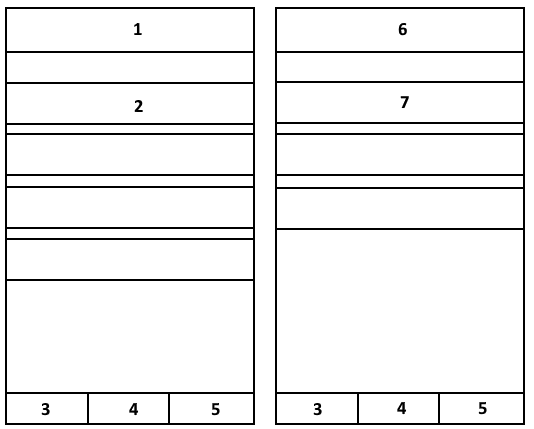
\includegraphics[width=0.55\linewidth]{vartotojo-sasaja.png}
	\caption{Akcijų kainų ir vartotojo aplanko atvaizdavimas}
	\label{fig:sas1}
\end{figure}

Paveikslėlyje \ref{fig:sas1} yra pavaizduotas akcijų kainų ir vartotojo aplanko modelis, kuris yra suskirstytas į skirtingas dalis, kurios atstoja skirtingą funkcionalumą. Kairiajame paveikslėlyje yra atvaizduojamos akcijos, kurias įvedžiau pats, ir naujų akcijų pridėti į sarašą yra neleidžiama. 1 - laukas yra skirtas lango pavadinimui ir sąrašo atnaujinimo funkcionalumui. 2 - sąrašo laukas skirtas sutrumpintiems akcijoms duomenims saugoti. Dešiniajame paveikslėlyje yra atvaizduojamas vartotojo aplankas į kurį vartotojas gali pridėti naujų akcijų. 6 - laukas skirtas lango pavadinimui, bei naujų akcijų pridėjimui į vartotojo akcijų sąrašą.7 - vartotojo akcijų sąrašo laukas, kuris atvaizduoja sutrumpintus akcijos duomenis. 3 - naršymo juostos liečiamas laukas, skirtas pereiti į iš anksto nustatytų akcijų sarašą. 4 - naršymo juostos liečiamas laukas skirtas pereiti į vartotojo akcijų aplanko langą. 5 - naršymo juostos liečiamas laukas skirtas pereiti į valiutų keitimo langą.

\newpage
\begin{figure}[h]
	\centering
	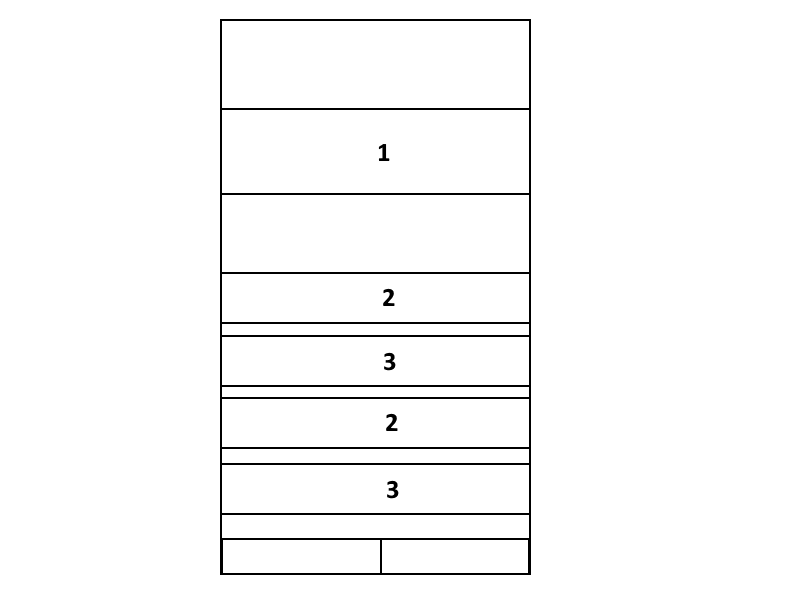
\includegraphics[width=0.55\linewidth]{vartotojo-sasaja2.png}
	\caption{Akcijų kainų ir vartotojo aplanko atvaizdavimas}
	\label{fig:sas2}
\end{figure}
Paveikslėlyje \ref{fig:sas2} kairėje yra pavaizduotas detalusis akcijos langas, į kurį patenkama paspaudus ant akcijos, o dešinėje pavaizduotas valiutos keitimo langas. Kairiajame paveikslėlyje 1 - lango pavadinimas ir grįžimas į bendrą akcijos peržiūros langą arba vartotojo aplanką priklausomai nuo to iš kur buvo įvykdyta naršymo komanda. 2 - valdymo juosta, kuri nurodo kuriam laikotarpiui atvaizduoti akcijos istorinį grafiką. 3 - akcijos istorinis grafikas, kuris atvaizduoja pasirinkto dienų laikotarpio akcijos kainas. 4 - pasirinktos akcijos detalesnių duomenų sąrašas. Dešiniajame paveikslėlyje 5 - valiutos keitimo lango pavadinimas. 6 - valiutos įvesties ir išvesties laukai. 7 - valiutos pasirinkimo langai, kurie atidaro nauja langą su valiutų pasirinkimais.

\newpage
\section{Praktinis programėlės įgyvendinimas}
Norint įgyvendinti mobilią akcijų stebėjimo sistemą man pirmiausia reikėjo išsiaiškinti, kur galiu gauti nemokamus ir patikimus akcijų duomenis.
\subsection{Technologijų pasirinkimas}
Programėlei realizuoti pasirinkau „Facebook“ įmonės sukurtą „JavaScript“ programavimo kalbos „React Native“ biblioteką. Programos paleidimui, kompiliavimui ir versijavimui pasirinkau nepriklausomų programuotojų sukurtą nemokamą produktą „Expo SDK“. Savo programėlę testavau nemokama „Android“ modeliavimo programa – „Genymotion“. Naršymą programėlės viduje įgyvendinau pasitelkdamas „React Navigation“ įrankį. Įvairių komponentų dalių ir būsenų išsaugojimą ir pernešimą programėlės viduje įgyvendinti pasitelkiau „Redux“ įrankį.
\subsubsection{„Expo SDK“ platforma}
Kuriant šią programėlę, man buvo labai svarbu kuo labiau supaprastinti programėlės kompiliavimo ir versijavimo procesą. Tam, kad nereikėtų nuolatos keisti kompiliavimo ir programėlės sudarymo proceso rankiniu būdu pasirinkau „Expo SDK“, kaip platformą savo programėlei. Ši platformą labai palengviną programėlės kompiliavimo ir kūrimo procesą automatiškai konfigūruodama kompiliavimą kiekvieną kartą pakeitus programinį kodą. Programuojant šioje platformoje man tapo prieinamas būdas naudoti „React Native“ biblioteką ir visą programą parašyti „JavaScript“ kalba be jokių sudėtingų kompiliatoriaus konfigūracijų. Ši platforma tapo labai naudinga tuo, kad ją įrašius iškarto galima naudotis daugybe integruotų bibliotekų, tokių, kaip pastarasis „React Native“, įvairios dizaino ir funkcionalumo bibliotekos. Taip pat ši platforma labai patogi darbui su "Android" sistema dėl integruotų įrankių, kurie leidžia kompiliutą kodą iškart atvaizduoti mobilioje sistemoje ir atnaujinti vos atnaujinus programinio kodo dalį.
\subsubsection{„React Native ir Redux“}
Funkcionalumui įgyvendinti pasirinkau „React Native“ programavimo kalbą. Ši programavimo kalba yra paremta savaisiais(ang. Native) mobiliųjų įrenginių programiniais kodais ir subendrina programavimą kelioms skirtingoms platformoms iš karto. Ši programavimo kalba yra sukurta, kaip „JavaScript“ kalbos biblioteka. Kadangi mano programėlėje yra būtinas bendravimas tarp skirtingų komponentų ir informacijos dalijimasis nusprendžiau tai įgyvendinti naudodamasis „Redux“ biblioteka. Ši biblioteka leidžia lengvai valdyti aplikacijos atmintyje laikomas savybes ir komponentų parametrus ir juos perduoti kitiems komponentas esantiems ne būtinai tame pačiame lygmenyje ar tame pačiame navigacijos lygyje.
\subsubsection{„Genymotion“}
Programėlės testavimui pasirinkau nemokamą modeliavimo įrankio „Genymotion“ versiją. Šis įrankis leidžia sukompiliuotą kodą atvaizduoti sumodeliuotame „Android“ įrenginyje kaskart atnaujinus programinį kodą. Taip smarkiai padidinamas programavimo darbo našumas, nes testavimas gali vykti ypatingai greitai ir nėra būtinybės programėlės testuoti tikrame įrenginyje.
\subsection{Išorinių duomenų šaltinių pasirinkimas}
Pasirinkau apjungti kelis skirtingus duomenų šaltinius, nes visi suteikė skirtingo funkcionalumo. „Yahoo Stocks API“ naudojau pagrindinių akcijų duomenų gavimui. Ši paslaugų tiekimo tarnyba ją kviečiant su norimu akcijos simboliu grąžina sąrašą duomenų apie pasirinktą akciją. Istoriniams akcijų pakitimų grafikams atvaizduoti naudojau „Quandl“ servisą, kuris grąžiną akcijų kainas pasirinktam laikotarpiui. Gautiems istoriniams kainų pakitimų grafikams atvaizduoti naudojausi išorine paslauga „HighCharts“. Ši paslauga leidžia atvaizduoti norimus duomenis pasirinktais grafikais, kurie pasirenkami siunčiant sukurtą konfigūraciją į išorinį paslaugų tiekėją.
\subsection{Sistemos struktūra}
Kuriant mobilią aplikaciją su „React Native“ ir „Redux“ technologijomis yra labai svarbu tinkamai struktūrizuoti projektą. Toliau pateiksiu mano sistemos struktūros pseudokoda:
\begin{itemize}[noitemsep]
\item komponentai
	\begin{itemize}[noitemsep]
		\item namų/
		\item portfelis/
	\end{itemize}
\item papildiniai/
\item konstantos/
	\begin{itemize}[noitemsep]
		\item isoriniai-servisai/
	\end{itemize}
\item redux/
	\begin{itemize}[noitemsep]
		\item reducers
		\item sore
	\end{itemize}
\item naršymo-maršrutai/
\item aplikacijos-pradžios-failas
\end{itemize}

Programai pradėjus darbą pirmiausia yra kreipiamasi į failą \textit{aplikacijos-pradžios-failas} kuris yra tėvinis projekto failas. Šis failas sukuria programoje naudojamus komponentus ir užregistruoja pradinę aplikacijos būseną, kuri vėliau yra naudojama saugoti parametrams, kurie yra perduodami skirtingose aplikacijos vietose esantiems komponentams. Pradinis sistemos būsenos registravimas vyksta aplanke \textit{redux/store.js}, o atskirų komponentų būsenos surenkamos \textit{redux/reducers.js}. Tuomet yra kreipiamasi į aplanką \textit{naršymo-maršrutai/}, kuris nusako, koks turi būti pirmasis komponentas, kurį sistema priima ir atvaizduoja vartotojui. Pirmasis komponentas kurį įkelia mano sistema yra failas \textit{komponentai/namų}. Tam, kad šis komponentas galėtų atvaizduoti mano norimą informaciją, buvo privaloma gauti pradinius naršymo maršrutų, programos būsenos ir išorinių servisų duomenis. Galiausiai namų komponente yra kviečiami išoriniai servisais iš ansčiau nurodyto failo ir viskas yra saugoma programos globalioje būsenoje.

\newpage
\section{Pagrindinio funkcionalumo įgyvendinimas}
Programėlės funkcionalumas susideda iš daugelio nedidelių funkcinių modulių, kurie yra paskirti atlikti tam tikrą veiksmų seką ir daugeliu atvejų grąžinti vienokį ar kitokį rezultatą. Funkcionalumai susiję su akcijų gavimu ir apipavidalinimu yra kuriami taikant teorines žinias perskaičius ~\cite{IGR} ir ~\cite{JOA} šaltinius, bei išanalizavus panašias programėles. Šiame skyriuje detaliau aptarsiu pagrindinius funkcionalumus ir kaip juos įgyvendinau.
\subsection{Vartotojo akcijų aplanko kūrimas}
Vienas pagrindinių programėlės funkcionalumų yra vartotojo akcijų aplanko kūrimas (pavaizduota priede E). Šis funkcionalumas yra pasiekiamas \textit{/areas/portfolio/PortfolioScreen.js}. Šiame lange yra pateikiamas akcijų sąrašas, kurias vartotojas pridėjo naudodamasis pliuso mygtuką. Paspaudus mygtuką yra atidaroma funkcija \textit{fetchSingleStocks(item)}. Ši funkcija priima vartotojo įvestą raktažodį ir vykdo pseudokodą (pavyzdys išeities kode \ref{code:fetchSingleStocks}). Pavyzdžio antrojoje eilutėje pavaizduotas išorinis paslaugų tiekėjas, kuriam pateikus norimos akcijos trumpinį yra grąžinamas duomenų apie akciją sąrašas. Šis sąrašas tuomet yra trečiojoje eilutėje interpretuojamas kaip objektas. Galiausiai ketvirtojoje eilutėje gautas objektas yra siunčiamas į aplikacijos atmintį(ang. state) ir ten yra išsaugomas vėlesniam panaudojimui.
\begin{lstlisting}[caption={Funkcijos fetchSingleStocks() pseudokodas.},label={code:fetchSingleStocks}]
fetchSingleStocks(akcijos-trumpinys) {
  const atsakas = gauti('http://d.yimg.com/aq/autoc?query=${akcijos-trumpinys}&region=US&lang=en-US')
  const atsakasJson = atsakas.json();
  nustatomeGlobaliaBusena({ paieskos-rezultatai: atsakasJson.akcija })	
}
\end{lstlisting}

Įvykdžius funkciją \textit{fetchSingleStocks(item)} programėlės atmintyje turiu naują akcijos objektą. Tam, kad šį objektą atvaizduočiau pridedu į sarašą naudodamasis „React Native“ komponentu \textit{ListView}. Šis komponentas priima objektą ir perduoda šį objektą į funkciją \textit{renderRow(item)}. Ši funkcija leidžia apdoroti vieną sarašo eilutę su gautais duomenimis ir grąžinti eilutę sąrašui. Tada yra kviečiama funkcija \textit{fetchYahooSingle(pasirinktasSimbolis)}, kuri ieško pasirinkos akcijos „Yahoo Finance“ duomenų bazėje (pavyzdys išeities kode \ref{code:fetchYahooSingle}). Antrojoje eilutėje kviečiamas išorinis servisas, kuris radęs akciją ją grąžina kaip masyvą. Toliau šeštoje eilutėje vykdome tikrinimą ar akcija yra grąžinta ir turi reikiamus duomenis. Jeigu akcija turi reikiamus duomenis aštuntoje eilutėje tikriname ar mūsų aplikacija jau turi tokią akciją savo būsenoje. Jeigu neturi, penkioliktoje eilutėje pridedame akciją į programėlės atmintį. Pats svarbiausias žingsnis yra septynioliktoje eilutėje, čia išsaugome rastą naują akciją į mobilaus prietaiso atmintį. Atlikus septynioliktą žingsnį ir perkrovus aplikaciją, vartotojas portfelio lange rastų išsaugotą akciją.

\newpage
\begin{lstlisting}[caption={Funkcijos fetchYahooSingle() pseudokodas.}, label={code:fetchYahooSingle}]
fetchYahooSingle(pasirinktasSimbolis) {
  const atsakas = gauti('https://query.yahooapis.com/v1/public/yql?q=select * from yahoo.finance.quotes where symbol in ( ${pasirinktasSimbolis} )&format=json&env=store/datatables.org/Falltableswithkeys&callback=')
  
  const atsakasJson = atsakas.json();
  const portfelis =  this.state.portfolio;
  if (atsakasJson nera tuscias ir turi duomenis 'open/ask') {
	  let rastasPortfelyje = [];
	  for(sukame cikla per 'portfelis' ir ieskome ar nera jau tokio simbolio) {
	   rastasPortefyle.push(atsakasJson);
	  }
  }
  
  if(rastasPortfelyje === 0) {
	  portfolio.push(atsakasJson)
	  nustatomeGlobaliaBusena({ portfelis: atsakasJson });
	  
	  AsyncStorage.setItem('portfelis');
  } 
  else {
	  Alert('Tokia akcija jau yra sarase!');
  }
}
\end{lstlisting}

Norint atnaujinti vartotojo akcijų portfelio sarašą yra kviečiama funkcija \textit{fetchYahooRefresh(portfelis)}. Ši funkcija kviečia išorinį servisą tiek kartų, kiek yra akcijų vartotojo portfelyje ir gauną atitinkamą kiekį masyvų. Kiekvieną masyvo elementas yra patikrinamas ar yra ne tuščias ir ar yra gauti atitinkami duomenys akcijai sėkmingai atvaizduoti. Jeigu duomenys yra gauti, senasis vartotojo portfelis yra ištrinamas iš programėlės atminties ir iš telefono atminties. Tuomet yra iš naujo išsaugojamas. Taip yra išvengiama pasikartojančių duomenų ir gaunami naujausi akcijų duomenys.

\subsection{Akcijos išplėsto turinio lango kūrimas}
Kiekviena akcija turi daugiau duomenų negu yra pavaizduota pagrindiniame ar vartotojo portfelio lange. Paspaudus ant vienos iš šių akcijų vartotojas yra nukreipiamas į išplėstą akcijos turinio langą (pavyzdys priede H). Perėjus į šį langą yra kviečiama funkcija \textit{fetchHistoricalData(akcijosSimbolis, dataIki, siandienosData)}. Ši funkcija kviečia išorinį servisą „QUANDL“, kuris pagal pateiktus duomenis: akcijos simbolį, pradžios datą ir pabaigos datą, gražina istorinius akcijos duomenis. Šie duomenys yra tokie, kaip kiekvienos dienos akcijos kaina rinkos atsidarymo, užsidarymo metu. Gauti duomenys yra įrašomi į programėlės atmintį ir yra kviečiamas kitas modalinis langas \textit{ChartScreen}. Šis langas atlieka grafiko atvaizdavimo funkcionalumą su duomenimis gautais iš \textit{fetchHistoricalData} funkcijos. Šiame lange yra sudaroma grafiko konfigūracija, nustatomos ašys: x - datų masyvas, y - didžiausios ir mažiausios kainos masyvai. Tuomet yra kviečiama funkcija \textit{highCharts}, kuri iš išorinio paslaugų tiekėjo gražina istorinį akcijos grafiką. Jeigu grafikas gražintas sėkmingai šiame lange aprašau grafiko aukštį ir plotį ir siunčiu atgal į išplėsto akcijos turinio langą. Grįžus į minėtajį langą yra atvaizduojamas gautas grafikas ir iš pagrindinio arba vartotojo profilio lango gauti išplėsti akcijos duomenys. Taip pat sukūriau grafiko datos imties keitimo funkcionalumą, kuris yra išdėstytas keturiais mygtukais virš grafiko. Kai yra paspaudžiamas vienas iš mygtukų, programėlės atmintyje pasikeičia laikinasis parametras nusakantis aktyvią grafiko datą, ir įvedant naująją vėl yra kreipiamasi į \textit{ChartScreen} langą ir yra atnaujinamas išplėstinis akcijos duomenų langas nauju grafiku. Kadangi yra kviečiami skirtingi duomenų tiekėjai grafikams ir akcijos duomenims atvaizduoti, būna atvejų kai yra negaunami vieni ar kiti duomenys.

\subsection{Valiutos keitimo lango kūrimas}

\begin{figure}[h]
	\centering
	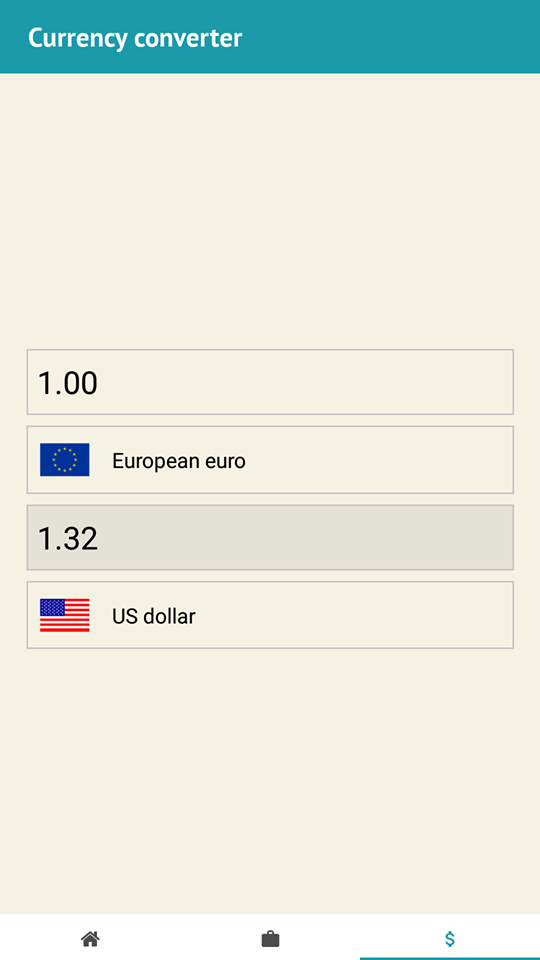
\includegraphics[width=0.3\linewidth]{currency.png}
	\caption{Valiutų keitimo langas}
	\label{fig:currency}
\end{figure}

Valiutos keitimo funkcionalumo įgyvendinimas man atrodė būtina dalis, nes ne visi vartotojai naudoja vienodą valiutą akcijoms stebėti ir pirkti (lango pavyzdys paveikslėlyje \ref{fig:currency}). Todėl buvo būtina užduotis sukurti būdą vartotojams išsiversti akcijų kainas į sau priimtiną valiutą. Šiame lange yra keturi laukai. Pirmasis laukas atlieka sumos įvedimo funkcionalumą (pavaizduota išeities kode \ref{code:calculateRate}). Šioje funkcijoje gavęs įvesties sumą, kursą ir išvesties kursą paskaičiuoju išvesties sumą. Išvesties suma yra atvaizduojama \textit{pav. \ref{fig:currency}} trečiame laukelyje ir šis laukelis yra skirtas tik išvesties atvaizdavimui. Taip pat yra galimybė keisti valiutas paspaudus ant laukų kurie pažymėti valiutų vėliavomis. Valiutos iš kurių sąrašo galima rinktis yra įkoduotos aplikacijoje.

\begin{lstlisting}[caption={Funkcijos calculateRate() pseudokodas.},label={code:calculateRate}]
calculateRate(ivestis, ivestiesKursas, isvestiesKursas) {
  const kursas = ivestiesKursas / isvestiesKursas;
  return (ivestis * kursas);
}
\end{lstlisting}

Valiutų kursai yra apskaičiuojami naudojantis išoriniu \textit{„Bank of Canada“} teikiamu, kasdien atnaujinamu duomenų sąrašu. Valiutų kursams gauti sukūriau funkciją \textit{fetchRates} (pavaizduota išvestie kode \ref{code:fetchRates}). Šioje funkcijoje yra kviečiamas išorinis duomenų tiekėjas ir gauti duomenys yra grąžinami masyvo formatu ir išsaugomi programėlės atmintyje iki kol valiutų keitimo langas yra atidaromas iš naujo.

\begin{lstlisting}[caption={Funkcijos fetchRates() pseudokodas.},label={code:fetchRates}]
fetchRates() {
 const valiutuKursai = fetch('http://www.bankofcanada.ca/valet/observations/group/FX_RATES_DAILY');
 const valiutuKursaiJson => {
   valiutuKursai.foreach((elementas) => {
	   return elementas.valiutosKodas;
   });
 }
}
\end{lstlisting}

 %Conclusions section
\sectionWithoutNumber{\keyWordConclusions}{conclu}
Šiame darbe buvo siekiama sukurti programėlę, kuri vartotojams suteiktų informaciją apie naujausius akcijos rinkų kainų pokyčius. Pagrindinis programėlės tikslas buvo suprogramuoti akcijų kainų stebėjimo sistemą, kur vartotojai patys galėtų pasirinkti norimas akcijas pateikę akcijos simbolį. Taip pat buvo siekiama, kad vartotojai turėtų papildomą valiutų keitimo funkcionalumą, bei galėtų detaliau apžiūrėti kiekvienos akcijos duomenis ir grafinius akcijos kainų pakitimus. Sukurtos programėlės funkcionalumai yra:
\begin{itemize}
	\item Vartotojo akcijų portfelio kūrimas pasirenkant norimą akcijos simbolį.
	\item Programėlėje įkoduotų akcijų simbolių atvaizdavimas.
	\item Akcijų sąrašų atnaujinimas ir išsaugojimas į mobilaus įrenginio atmintį.
	\item Akcijos kainos pasikeitimų per nustatytą laiką grafinis atvaizdavimas ir detalus akcijos duomenų atvaizdavimas.
	\item Valiutų keitimas.
\end{itemize}
Rekomendacijos tolesniam darbo vystymui:
\begin{itemize}
	\item Apjungti išorinius duomenų tiekėjus į vieną, tam, kad nebūtų duomenų paklaidų ir būtų optimizuotas paieškos, bei atvaizdavimo greitis.
	\item Sukurti interaktyvų akcijų pirkimo ir pardavimo žaidimą.
\end{itemize}


%file literatureSources.bib
\referenceSources{literatureSources}

%% this part is optional
\newpage
\begin{appendices}
	
\begin{figure}[h!]
	\centering
	\begin{subfigure}{0.5\textwidth}
		\centering
		\tocless\section{Programėlė „My Stocks Portfolio and Widget“}
		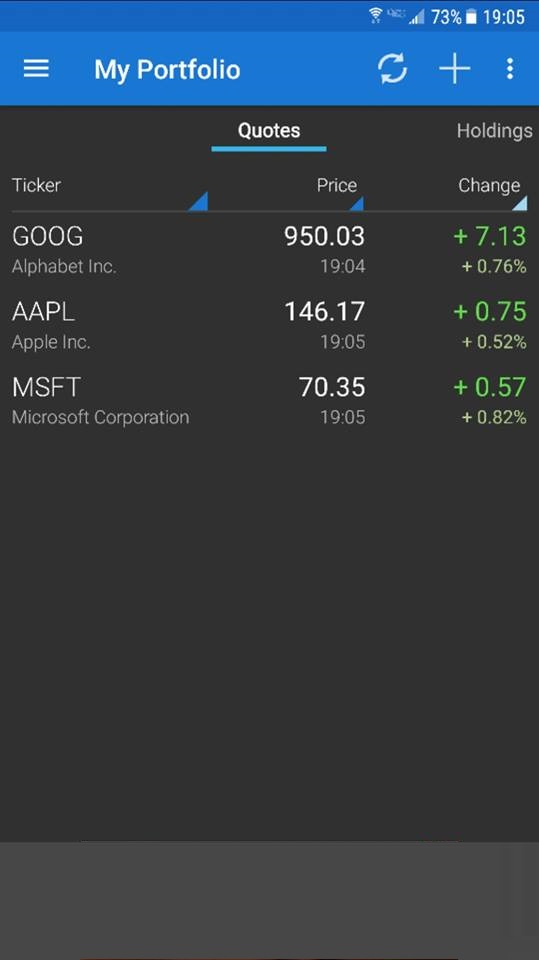
\includegraphics[scale=0.532]{priedas1.jpg}
		\label{app:priedas1}
	\end{subfigure}%
	\begin{subfigure}{0.5\textwidth}
		\centering
		\tocless\section{Programėlė „My Stocks Portfolio and Widget“}
		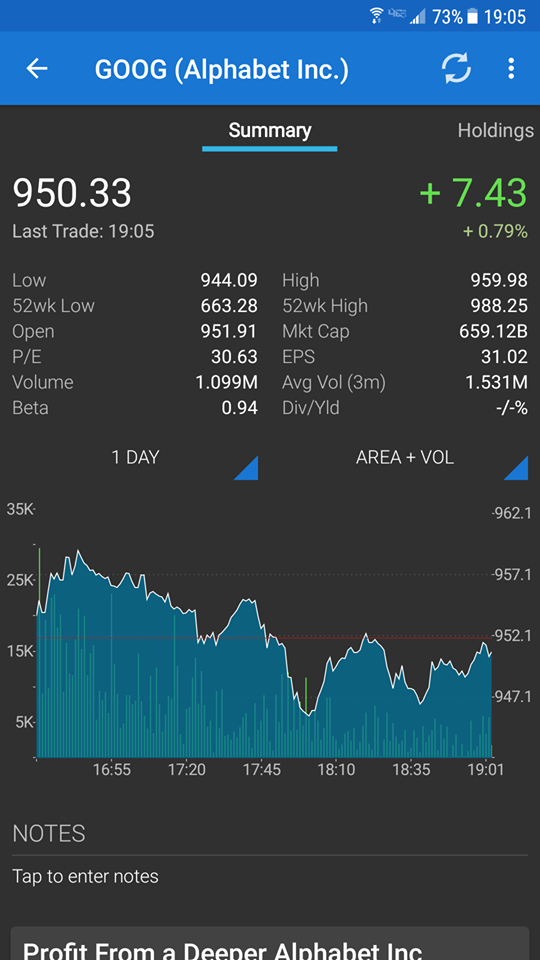
\includegraphics[scale=0.4]{priedas2.png}
		\label{app:priedas2}
	\end{subfigure}
\end{figure}
\begin{figure}[h!]
	\centering
	\begin{subfigure}{0.5\textwidth}
		\centering
		\tocless\section{Antroji analizuota aplikacija}
		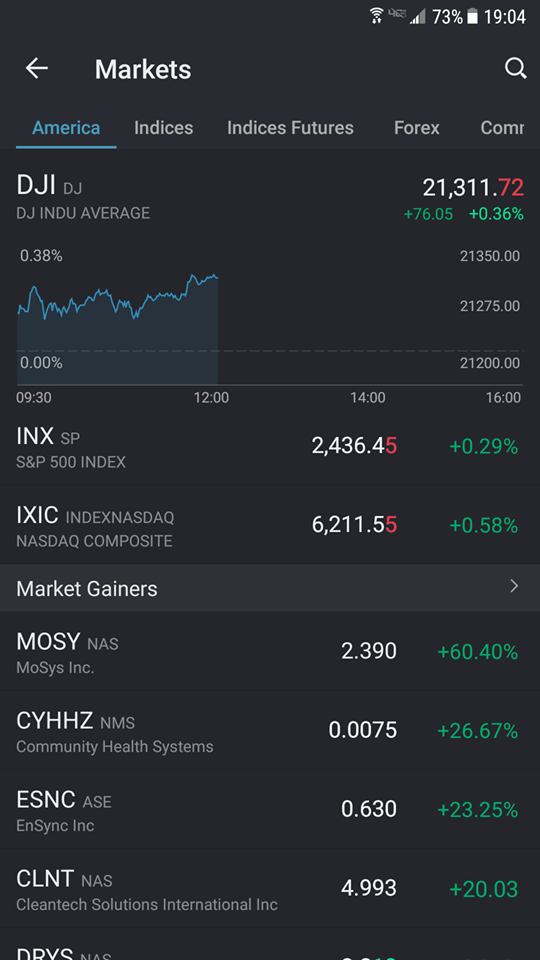
\includegraphics[scale=.4]{priedas3.png}
		\label{app:priedas3}
	\end{subfigure}%
	\begin{subfigure}{0.5\textwidth}
		\centering
		\tocless\section{Antroji analizuota aplikacija}
		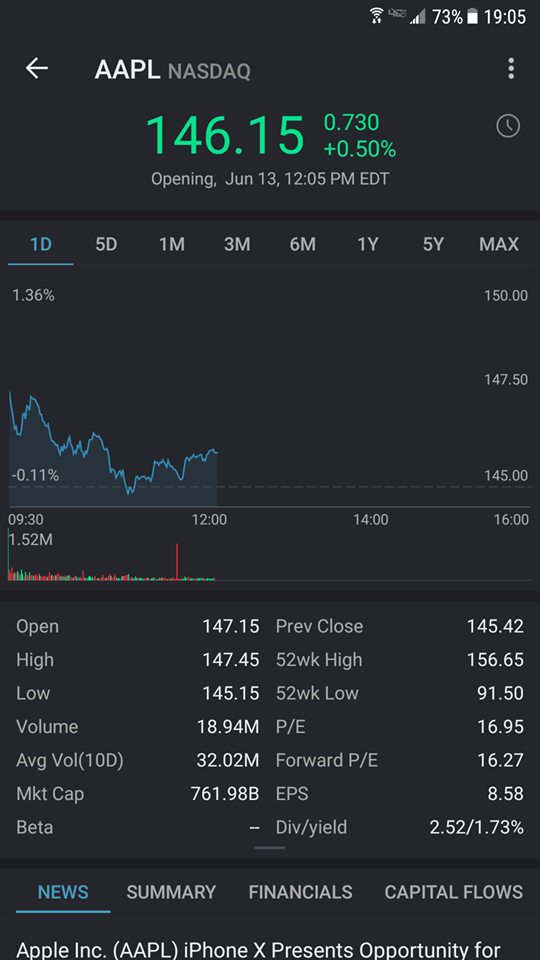
\includegraphics[scale=0.4]{priedas4.png}
		\label{app:priedas4}
	\end{subfigure}
\end{figure}

\begin{figure}
	\begin{subfigure}{0.5\textwidth}
		\centering
		\tocless\section{Vartotojo akcijų portfelio langas}\label{app:priedas5}
		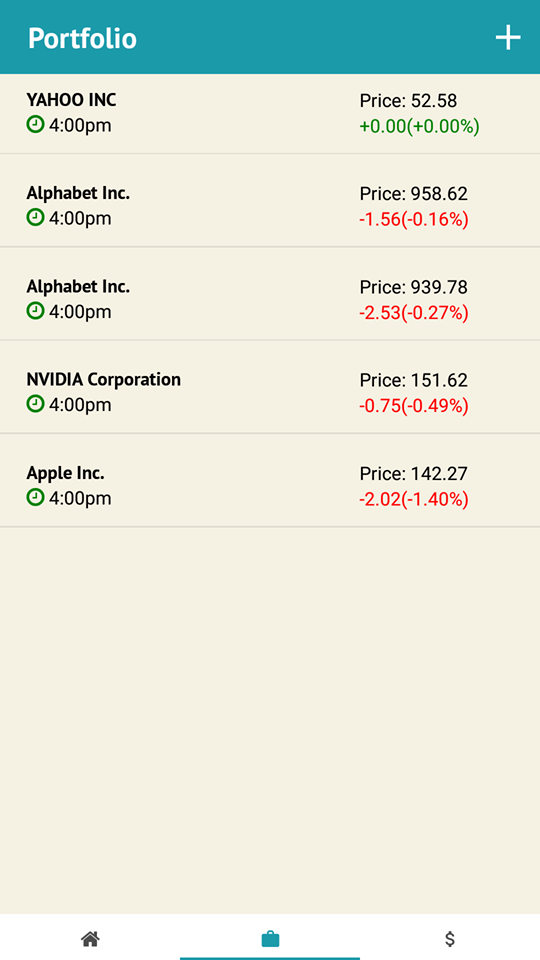
\includegraphics[width=0.8\linewidth]{portfolio.png}
	\end{subfigure}%
	\begin{subfigure}{0.5\textwidth}
		\centering
		\tocless\section{Akcijos paieškos laukas portfelio lange}
		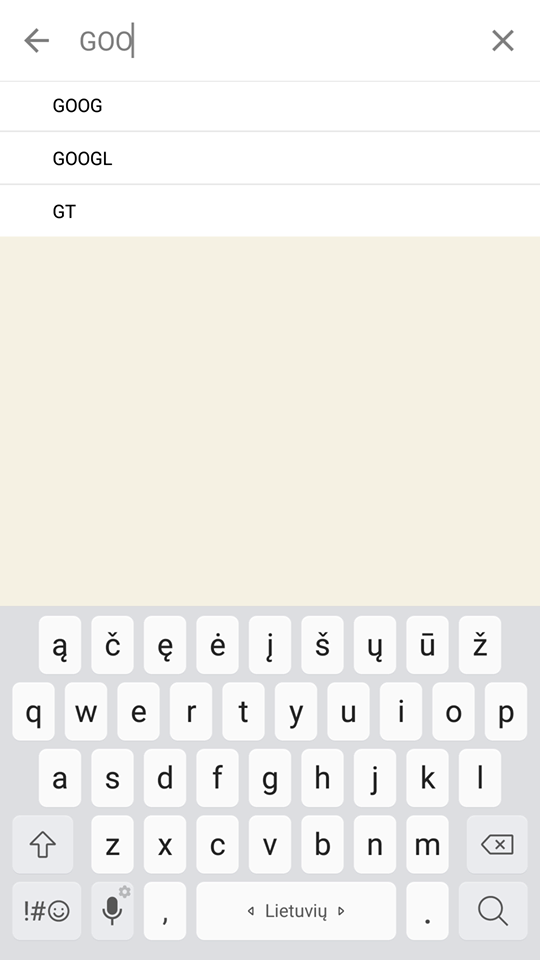
\includegraphics[width=0.8\linewidth]{stockSearch.png}
		\label{app:priedas6}
	\end{subfigure}
\end{figure}

\begin{figure}
	\begin{subfigure}{0.5\textwidth}
		\centering
		\tocless\section{Pradinis programėlės akcijų langas}
		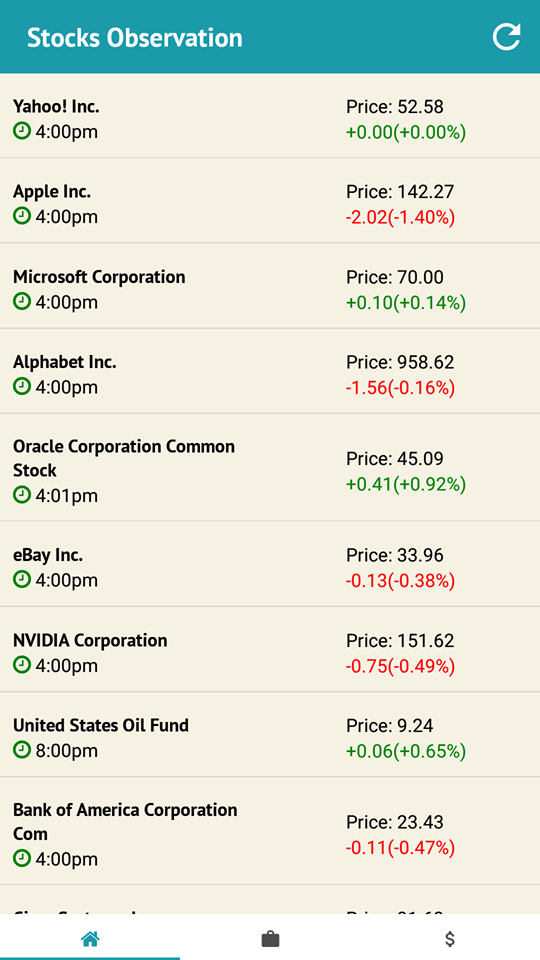
\includegraphics[width=0.8\linewidth]{home.png}
		\label{app:priedas7}
	\end{subfigure}
	\begin{subfigure}{0.5\textwidth}
		\centering
		\tocless\section{Akcijos duomenų detalaus atvaizdavimo langas}
		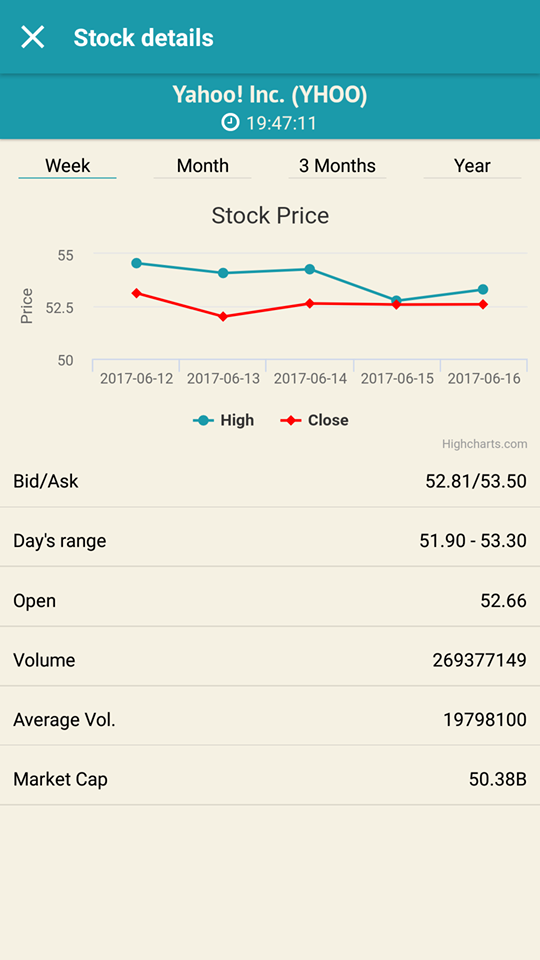
\includegraphics[width=0.8\linewidth]{stockDetails.png}
		\label{app:priedas8}
	\end{subfigure}%
\end{figure}

\end{appendices}


\end{document}
